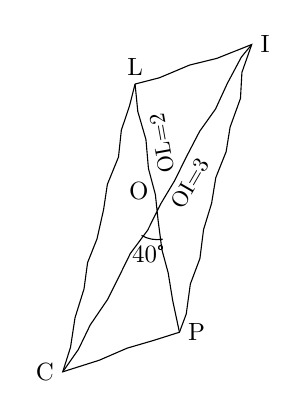
\begin{tikzpicture}[rotate=60,every node/.style={scale=0.9},scale=0.8]

\coordinate (C) at (0,0);
\coordinate (L) at (4.53,1.29);
\coordinate (I) at (6,0);
\coordinate (P) at (1.47,-1.29);
\coordinate (O) at (3,0); %le centre du parallélogramme

\draw[decorate,decoration={random steps,amplitude=1pt,segment length=10pt}] (C) node [left]{C}--(L) node [above]{L}--(I) node [right] {I}--(P) node [right] {P}--cycle;

\draw [decorate,decoration={random steps,amplitude=1pt,segment length=10pt}] (C)--(I) (L)--(P);
\draw (2.5,0) arc (-180:-140:0.5);
\draw (2.3,-0.25) node {40°};
\draw (O) node [above left]{O};

\path (O)--(I) node[pos=0.2,below,sloped,scale=0.9,rotate=60]{OI=3};
\path (O)--(L) node[midway,below,sloped,scale=0.9,rotate=60]{OL=2};

\end{tikzpicture}

